\documentclass{beamer}
\mode<presentation>
\usetheme{CambridgeUS}
\usepackage[russian]{babel}
\usepackage[utf8]{inputenc}
\usepackage[T2A]{fontenc}
\usepackage{sansmathaccent}

\usepackage{verbatim}
\usepackage{alltt}

\pdfmapfile{+sansmathaccent.map}
\title[Software Design]{Введение в программную инженерию}
\author{Наумов Д.А., доц. каф. КТ}
\date[11.02.2019] {Основы программной инженерии, 2019}

\begin{document}

%ТИТУЛЬНЫЙ СЛАЙД
\begin{frame}
  \titlepage
\end{frame}
  
%СОДЕРЖАНИЕ ЛЕКЦИИ
\begin{frame}
  \frametitle{Содержание лекции}
  \tableofcontents  
\end{frame}
  
%РАЗДЕЛ 1
\section{История и основные понятия}

\begin{frame}[t]
\textbf{Программная инженерия} есть применение определенного систематического
измеримого подхода при разработке, эксплуатации и поддержке программного
обеспечения. 
\begin{itemize}
\item \textit{software} (программное обеспечение, ПО) - 1958, Джон Тьюкей (John Tukey)
\item \textit{software engineering} (программная инженерия) - конференция НАТО, Германия, 1968
\item c 1990 по 1995 год: работа над международным стандартом о процессах разработки ПО (ISO/IEC 12207)
\item  "Руководство к своду знаний по программной инженерии" (SWEBOK), 2004
\end{itemize}
\end{frame} 
   
\begin{frame}[t]
\textbf{Программирование} - процесс отображения определенного множества целей на
множество машинных команд и данных, интерпретация которых на компьютере
или вычислительном коплексе обеспечивает достижение поставленных целей. 
\begin{itemize}
\item цели $\rightarrow$ требования к системе
\item требования $\rightarrow$ высокоуровневая архитектура и спецификации компонентов
\item спецификации $\rightarrow$ на дизайн компонентов
\item дизайн $\rightarrow$ на исходный код 
\item исходный код $\rightarrow$ код развертывания
\item код развертывания $\rightarrow$ вызовы функций ПО окружения (ОС,
промежуточное ПО, базы данных), которое может располагаться на множестве
компьютеров, объединенных в сеть
\item вызовы функций ПО окружения $\rightarrow$ машинные команды и данные.
\end{itemize}
\end{frame} 

\begin{frame}[t]
\begin{block}{Профессиональное программирование}
деятельность, направленная на получение доходов при помощи
программирования. 
\end{block}
Профессиональное производство программ это всегда коллективная деятельность, в которой участвуют минимум два человека:
программист и потребитель.
\begin{block}{Профессиональный программист}
человек, который занимается профессиональным программированием. 
\end{block}
\end{frame}

\begin{frame}[t]
\begin{enumerate}
\item Сложность
\begin{itemize}
\item API, библиотеки компонентов, много составных частей
\item Алгоритмы и методы
\item Неспособность одного человека удержать все детали в голове
\end{itemize}
\item Необходимость реализовать «вчера» 
\item Низкое повторное использование кода
\item Необходимость интеграции с внешними системами
\item Распределенная и неоднородная среда
функционирования
\end{enumerate}
\end{frame}

\begin{frame}[t]
\begin{block}{Жизненный цикл ПО} 
время от идеи до вывода из эксплуатации. 
\end{block}
Основные этапы
\begin{itemize}
\item Разработка требований 
\item Анализ
\item Проектирование 
\item Разработка
\item Тестирование 
\item Внедрение
\item Эксплуатация 
\item Вывод из эксплуатации
\end{itemize}
ISO/IEC 12207-2008 “Information Technology – Software Life Cycle Processes” (ГОСТ Р ИСО/МЭК 12207-2010)
\end{frame}

\begin{frame}
Жизненный цикл программного продукта
\begin{figure}[h]
\centering
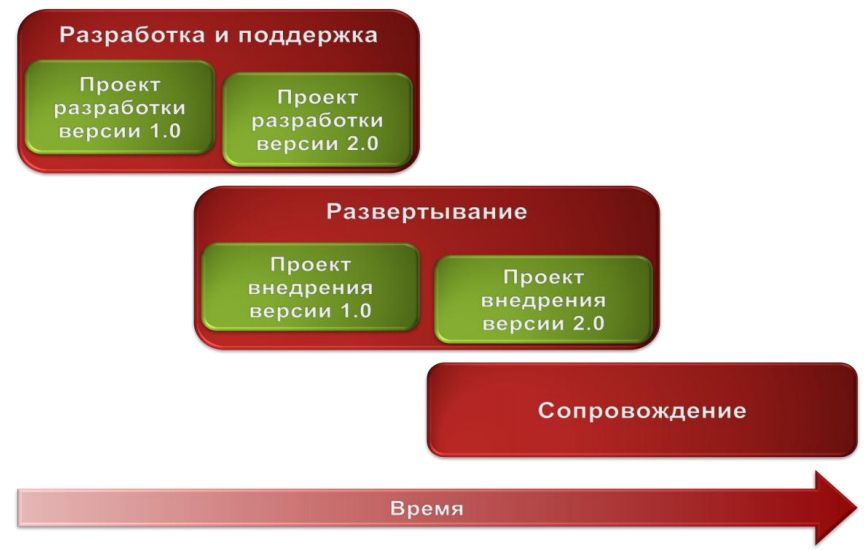
\includegraphics[scale=0.5]{images/lec01-pic01.png}
\label{pic-sort}
\end{figure}
\end{frame}

\begin{frame}[t]
\begin{block}{Процесс разработки ПО} 
совокупность процессов, обеспечивающих создание и развитие программного обеспечения. 
\end{block}
\begin{block}{Модель процесса разработки ПО}
формализованное представление процесса разработки ПО.
\end{block}
Часто при описании процессов вместо слова \textit{модель} употребляется термин \textit{методология}, что приводит к неоправданному расширению данного понятия. 
\end{frame}

\begin{frame}
Группы процессов ЖЦ (ISO/IEC 12207:2010)
\begin{figure}[h]
\centering
\includegraphics[scale=0.4]{images/lec01-pic05.png}
\label{pic-sort}
\end{figure}
\end{frame}

\begin{frame}[t]
Основные области знаний программной инженерии (согласно SWEBOOK 2004)
\begin{enumerate}
\item Software requirements – программные требования.
\item Software design – дизайн (архитектура).
\item Software construction – конструирование программного обеспечения.
\item Software testing – тестирование.
\item Software maintenance – эксплуатация (поддержка) программного обеспечения.
\item Software configuration management – конфигурационное управление.
\item Software engineering management – управление в программной
инженерии.
\item Software engineering process – процессы программной инженерии.
\item Software engineering tools and methods – инструменты и методы.
\item Software quality – качество программного обеспечения.
\end{enumerate}
\end{frame} 

\begin{frame}[t]
Дополнительные области знаний программной инженерии (согласно SWEBOOK 2004)
\begin{enumerate}
\item Computer engineering – разработка компьютеров.
\item Computer science – информатика.
\item Management – общий менеджмент.
\item Mathematics – математика.
\item Project management – управление проектами.
\item Quality management – управление качеством.
\item Systems engineering – системное проектирование.
\end{enumerate}
\end{frame} 

\section{Отличия программной инженерии от других отраслей}
\begin{frame}[t]
Результаты анализа успешности программных проектов за 2006 год
\begin{figure}[h]
\centering
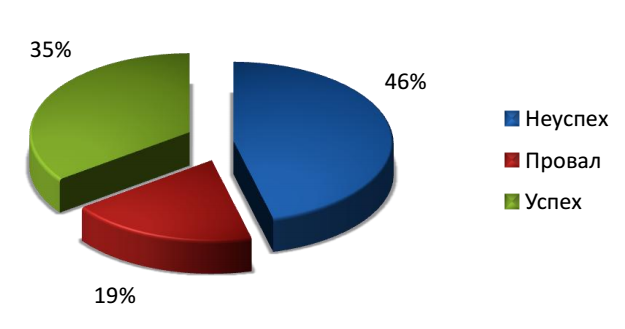
\includegraphics[scale=0.35]{images/lec01-pic02.png}
\label{pic-sort}
\end{figure}
\begin{itemize}
\item Только 35\% проектов завершились в срок, не превысили запланированный бюджет и реализовали все требуемые функции и возможности.
\item 46\% проектов завершились с опозданием, расходы превысили запланированный бюджет, требуемые функции не были реализованы в полном объеме.
\item 19\% проектов полностью провалились и были аннулированы до завершения.
\end{itemize}
Кто виноват? Что делать?
\end{frame} 

\begin{frame}[t]
\begin{block}{Ф. Брукс, 1975:} 
Программист, подобно поэту, работает почти непосредственно с чистой мыслью. Он строит свои замки шлифовки или переработки и доступен для воплощения грандиозных замыслов. 
\end{block}
\begin{itemize}
\item программирование - наука?
\item программирование - искусство?
\item программирование - ремесло?
\item программирование - сходство и отличия с другими областями знаний
\end{itemize}
\end{frame}

\section{Эволюция подходов к управлению}
\begin{frame}[t]
\begin{itemize}
\item \textit{Как получится}. Полное доверие техническим лидерам. Представители бизнеса практически не участвует в проекте. Планирование, если оно и есть, то неформальное и словесное. Время
и бюджет, как правило, не контролируются.
\item \textit{Водопад} или каскадная модель. Жесткое управление с обратной связью.
\item \textit{Гибкое управление}. Гибкое управление с обратной связью
\item \textit{Метод частых поставок}.
\end{itemize}
Классические методы управления перестают работать, когда:
\begin{itemize}
\item структура и свойства управляемого объекта нам не известны и/или изменяются со временем
\item рабочая группа проекта не может обеспечить требуемую эффективность
\end{itemize}
Когда структура и свойства управляемого объекта нам не известны, необходимо использовать адаптивное управление, которое, дополнительно к прямым управляющим воздействиям, направлено на изучение и изменение свойств управляемого объекта.
\end{frame}

\begin{frame}[t]
\begin{block}{Модель ЖЦ ПО} 
это структура, определяющая последовательность выполнения и взаимосвязи процессов, действий и задач на
протяжении всего ЖЦ. 
\end{block}
\begin{itemize}
\item Последовательная: определены все требования, один этап разработки
\item Инкрементная: определены все требования, несколько этапов
\item Эволюционная: определены не все требования, несколько этапов
\item Формальных преобразований
\end{itemize}
\end{frame}

\begin{frame}[t]
\begin{itemize}
\item Методологии разработки (Модель?, Метод?, Методология?)
\item Agile Unified Process (AUP), Behavior Driven
Development (BDD), Big Design Up Front (BDUF),
Design-driven development (D3), Disciplined Agile
Delivery (DAD), Dynamic Systems Development
Method (DSDM), Enterprise Unified Process (EUP),
Feature Driven Development (FDD), Lean software
development, Microsoft Solutions Framework (MSF),
Model-driven architecture (MDA), Open Unified
Process, Outside In Development (OID) Rapid
application development (RAD), Rational Unified
Process (RUP), Scrum, Spiral model, Unified Process
(UP), V-Model, Waterfall model
\end{itemize}
\end{frame}

\begin{frame}
Различные модели процесса разработки ПО и их распределение по "весу"
\begin{figure}[h]
\centering
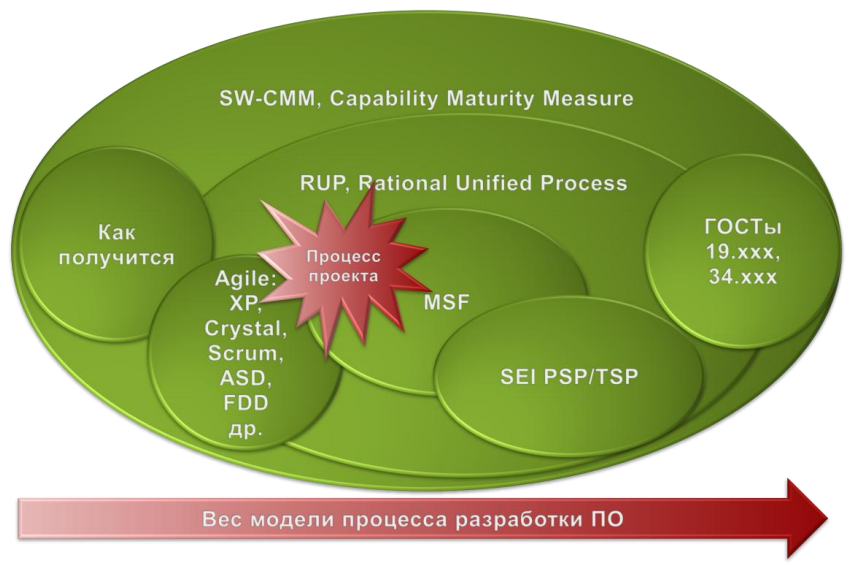
\includegraphics[scale=0.5]{images/lec01-pic03.png}
\label{pic-sort}
\end{figure}
\end{frame}

\begin{frame}[t]
ГОСТы (ГОСТ 19 "Единая система программной документации" и ГОСТ 34 "Стандарты
на разработку и сопровождение автоматизированных систем")
\begin{itemize}
\item ориентированы на последовательный подход к разработке ПО
\item разработка проводится по этапам, каждый из которых предполагает выполнение строго определенных работ, и завершается выпуском достаточно большого числа весьма формализованных и обширных документов
\item строгое следование не только приводит к водопадному подходу, но и требует очень высокой степени формализованности разработки.
\item на основе этих стандартов разрабатываются программные системы по госзаказам в России.
\end{itemize}
\end{frame}

\begin{frame}[t]
SW-CMM (Capability Maturity Model for Software)
\begin{itemize}
\item данная модель определяет пять уровней зрелости процесса разработки ПО (Начальный, Повторяемый, Определенный, Управляемый, Оптимизируемый).
\item документация с полным описанием занимает около 500 страниц и определяет набор из 312 требований, которым должна соответствовать организация, если она планирует аттестоваться по этому стандарту на 5-ый уровень зрелости.
\end{itemize}
\end{frame}

\begin{frame}[t]
RUP (Rational Unified Process)
\begin{itemize}
\item разработан в качестве дополнения к языку моделирования UML
\item описывает абстрактный общий процесс, на основе которого организация или проектная команда должна
создать конкретный специализированный процесс, ориентированный на ее потребности
\item можно использовать и как основу для самого что ни на есть традиционного водопадного стиля разработки, так и в качестве гибкого процесса
\end{itemize}
\end{frame}

\begin{frame}[t]
Microsoft Solutions Framework (MSF)
\begin{itemize}
\item это гибкая и достаточно легковесная модель, построенная на основе итеративной разработки
\item большое внимание к созданию эффективной и небюрократизированной проектной команды
\item предлагает достаточно нестандартные подходы к организационной структуре, распределению ответственности и принципам взаимодействия внутри команды
\end{itemize}
\end{frame}

\begin{frame}[t]
PSP/TSP (Personal Software Process / Team Software Process)
\begin{itemize}
\item делает ставку на самоуправляемые команды численностью 3–20 разработчиков
\item определяет требования к компетенциям команд в целом и программистов
\end{itemize}
Каждый программист должен уметь:
\begin{itemize}
\item учитывать время, затраченное на работу над проектом;
\item учитывать найденные дефекты и классифицировать типы дефектов;
оценивать размер задачи;
\item осуществлять систематический подход к описанию результатов
тестирования;
\item планировать программные задачи; распределять их по времени и составлять график работы.
\item выполнять индивидуальную проверку проекта и архитектуры;
\item выполнять регрессионное тестирование.
\end{itemize}
\end{frame}

\begin{frame}[t]
Agile (гибкая разработка ПО)
\begin{itemize}
\item применяемый в разработке ПО процесс должен быть адаптивным
\item высшей ценностью является ориентированность на людей и их взаимодействие, а не на процессы и средства
\item гибкие методологии это - набор практик, которые могут позволить (а могут и нет) добиваться эффективной разработки ПО, основываясь на итеративности, инкрементальности, самоуправляемости команды и адаптивности процесса.
\end{itemize}
\end{frame}

\begin{frame}
Процесс в проекте должен определяться в зависимости от проекта, продукта и персонала
\begin{figure}[h]
\centering
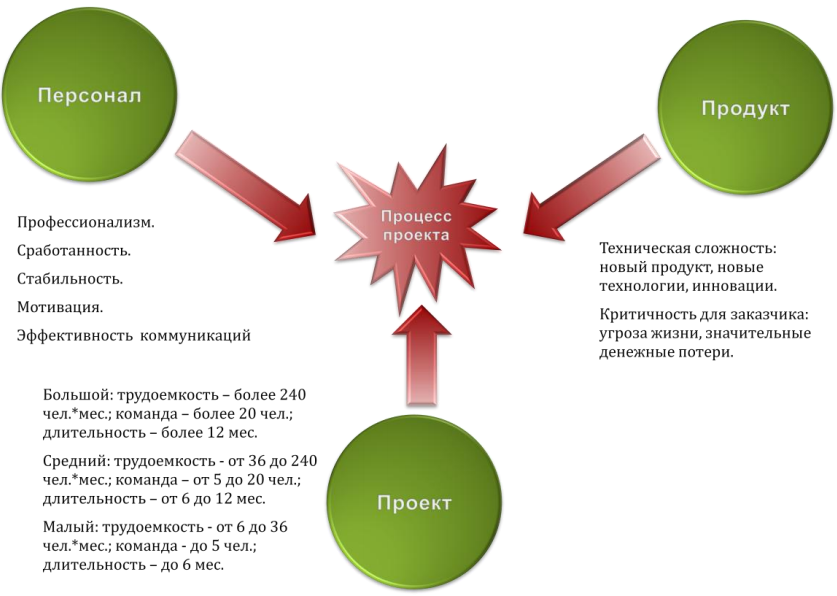
\includegraphics[scale=0.5]{images/lec01-pic04.png}
\label{pic-sort}
\end{figure}
\end{frame}

\begin{frame}
Что надо делать для успеха программного проекта? (Стив Макконнелл, «Остаться в живых. Руководство для менеджеров
программных проектов», «Питер», 2006)
\begin{enumerate}
\item Четко ставить цели.
\item Определять способ достижения целей.
\item Контролировать и управлять реализацией.
\item Анализировать угрозы и противодействовать им.
\item Создавать команду.
\end{enumerate}
\end{frame}

\begin{frame}
Выводы
\begin{itemize}
\item То, что производят программисты нематериально – это коллективные мысли и
идеи, выраженные на языке программирования. В силу уникальности отрасли
опыт, накопленный в отраслях материального производства, мало способствует
успеху в управлении программным проектом. Прямые аналогии с этими
отраслями не работают. Управлять разработкой ПО надо иначе.
\item Не существует единственного правильного процесса разработки ПО.
Эффективный производственный процесс должен основываться на
итеративности, инкрементальности, самоуправляемости команды и
адаптивности. Главный принцип: не люди должны строиться под выбранную
модель процесса, а модель процесса должна подстраиваться под конкретную
команду, чтобы обеспечить ее наивысшую производительность.
\end{itemize}
\end{frame}

\section*{Литература}
\begin{frame}   
\begin{enumerate}
\item IEEE Std 610.12-1990, IEEE Standard Glossary of Software Engineering Terminology.
\item EEE Std 1074-1995, IEEE Standard for Developing Software Life Cycle Processes.
\item "Руководство к своду знаний по программной инженерии". The Guide to the Software Engineering Body of Knowledge, SWEBOK, IEEE Computer Society Professional Practices Committee, 2004.
\item David Rubinstein, "Standish Group Report: There‘s Less Development Chaos Today". 2007 (http://www.sdtimes.com/content/article.aspx?ArticleID=30247)
\item Брукс Фредерик, "Мифический человеко-месяц, или Как создаются программные комплексы", Пер. с англ., СПб., Символ-Плюс, 1999 
\item "PMBOK. Руководство к Своду знаний по управлению проектами", 3-е изд., PMI, 2004.
\item Уолкер Ройс, "Адаптивный стиль управления программными проектами". Открытые системы. 2006. № 1.
\end{enumerate}
\end{frame}


\section*{Литература}
\begin{frame}   
\begin{enumerate}
\setcounter{enumi}{7}
\item Ершов А. П., "О человеческом и эстетическом факторе в программировании". Информатика и образование. 1993. № 6.
\item Paulk, Mark C., and others, Capability Maturity Model for Software, Version 1.1 (CMU/SEI-93-TR-24). Pittsburgh, Pa.: Software Engineering Institute, Carnegie Mellon University, 1993.
\item Филипп Крачтен, "Введение в Rational Unified Process", Вильямс, 2002 г.
\item "MSF, Microsoft, Microsoft Solutions Framework", Отдел MSF, Microsoft, 2002.
\item M. Pomeroy-Huff, J. Mullaney, R. Cannon, M. Sebern, "The Personal Software Process (PSP) Body of Knowledge", version 1.0, SPECIAL REPORT CMU/SEI, 2005
\item Watts S. Humphrey, "The Team Software Process (TSP)", Technical Report CMU/SEI, 2000
\item Kent Beck, and others, "Manifesto for Agile Software Development", 2001 (http://www.agilemanifesto.org/)
\end{enumerate}
\end{frame}

\begin{frame}   
\begin{enumerate}
\setcounter{enumi}{14}
\item А. Коуберн, "Люди как нелинейные и наиболее важные компоненты в создании программного обеспечения", Humans and Technology Technical Report, Oct.1999
\item А. Коуберн, "Каждому проекту своя методология", Humans and Technology Technical Report, TR 99.04, Oct.1999 (русский перевод К.Максимов, А.Максимова).
\item С. Макконнелл, "Остаться в живых. Руководство для менеджеров программных проектов", "Питер", 2006.
\end{enumerate}
\end{frame}

\end{document}
